\documentclass[UTF8]{gapd}
\usepackage{amsmath}
\usepackage{multirow}
\usepackage{float}
\usepackage{footnote}
%基础模板,引用自GitHub: https://github.com/RocketshipGames/gapd.cls

% ■ ■ ■ ■ ■ ■ ■ ■ ■ ■ ■ ■ ■ ■ ■ ■ ■ ■ ■ ■ ■ ■ ■ 
% ■ ■ ■ ■ ■ ■ ■ ■ ■ ■ ■ ■ ■ ■ ■ ■ ■ ■ ■ ■ ■ ■ ■
% ■ ■               注意事项                 ■ ■
% ■ ■      不要瞎几把模板里面cls文件!!!!!   ■ ■
% ■ ■      写着不需要改动的地方别瞎几把动!!!   ■ ■
% ■ ■      有不懂的地方就直接联系编辑!!!!!   ■ ■
% ■ ■      不要自作主张!!!!!!             ■ ■
% ■ ■      否则后续排版会非常累的!!!!!!!   ■ ■
% ■ ■ ■ ■ ■ ■ ■ ■ ■ ■ ■ ■ ■ ■ ■ ■ ■ ■ ■ ■ ■ ■ ■
% ■ ■ ■ ■ ■ ■ ■ ■ ■ ■ ■ ■ ■ ■ ■ ■ ■ ■ ■ ■ ■ ■ ■

%标题部分=================================================================
%上标(不需要改动!!!!)
\Type{Article}

%标题
\Title{
  水螺旋
}

\CAuthor{谭帆驰,鲍子龙}{IBPE2021}%显示于题目下的作者名,
\Author{Xing Ming}{}
%出现于页脚初的英文名,按“姓 名”的顺序写拼音

%摘要
\Abstract{本文是对于2022CUPT第九题研究成果的一个总结.理论上,作者考虑用柱坐标下的三维扰动对螺旋的产生进行解释,螺旋的形状体现在对$	\theta 	$的扰动上,本文通过不同的模式(参数$m$)对此进行表述.此外,作者对于不同模式的扰动定义了随时间发生变化的增长率$\alpha$,由此判断哪种模式将占主导地位,并由此预言将产生的螺旋形状.实验上,我们使用不同流速的同轴气体带来扰动,通过观察不同风速下产生的不同螺旋的形状来验证理论的合理性.}
\Keywords{扰动模式,同轴气体,螺旋形状,表面张力}
%编号与页码(以下两行不需要改动)
\Issue{1}{1}{2022}
\Pages{1}{3}%37
%不要改这里,好吗?

%正文部分=================================================================
\begin{document}
%\begin{CJK}{UTF8}{gbsn}
\maketitle

%一些常用的Latex语句:
%插入斜体:\textit{}
%引用文字:\begin{quote} \end{quote}
%插入脚标: \footnote{}

\section{简介}
\label{sec:Introduction}
\begin{quote}
	If \textcolor{red}{a stream of liquid} is launched through \textcolor{red}{a small hole}, then under certain conditions it \textcolor{red}{twists into a spiral}. Explain this phenomenon and investigate \textcolor{red}{the conditions under which the spiral will twist}.
	
	如果\textcolor{red}{一股液体}从\textcolor{red}{一个小孔}中射出,那么在一定条件下,它会扭转成\textcolor{red}{螺旋状}.解释这一现象,并研究\textcolor{red}{产生螺旋的条件}.
\end{quote}



%插入普通图片
\iffalse
\begin{figure}[!htbp]%
  \centering
  \includegraphics[width=0.8\columnwidth]{图片地址}
  \caption{图片名}
  \label{fig:P2}%\label置于\caption后,否则可能报错
\end{figure}
\fi%实际写时不需要\iffalse \fi,(该组命令是为了编辑时不报错)

%插入跨列图片
\iffalse
\begin{figure*}[!htbp]
  \centering
  \includegraphics[width=1\linewidth]{图片地址}
  \caption{图片名}
  \label{fig:P1}
\end{figure*}
\fi

%插入图表一定要注意规范!!!!!!!!!!!!!!!!!!!!!!!!!!!!!!!!!!!!!!
%表格一律用三线表,如果有出现数据,请注明数据的单位,另外表格的标题等也要注明清楚。

%插入任何非原创图片都应当注意注明出处
%插入一般的曲线图,一定要注明坐标轴的含义!!!!!及其单位!!!!!!  格式一律为:      物理量 (单位)
%                                                                              ^
%                                                                              |
%                                                                              |
%                                                                              |
%                                                                例子:         ——————————————————————————>
%                                                                                     摆线长度  (mm)
%当图中存在多个曲线,或者数据与拟合图同时存在时,要写清楚图例!!!!!!!!!
%要善于运用跨列图片,把多个相似的子图拼组合成一张比较大的跨列图片


\section{理论}
\label{sec:Theory}
\subsection{提出假设}

\begin{enumerate}
	\item 液体是不可压缩的,气体是不可压缩且无粘性的。
	\item \textbf{考虑三维扰动,在柱坐标系下表达为如下形式:}
	\begin{equation}
p_{i}=p_{i}(r) e^{i(k z+m \theta)+\alpha t} 
	\end{equation}
	\begin{equation}
	u_{i}=u_{i}(r) e^{i(k z+m \theta)+\alpha t}
	\end{equation}
	\item 假设液体与气体的密度比以及气体速度都是恒定值
\end{enumerate}

\subsection{模型建立}
\subsubsection{无黏情况}
暂时不考虑液体粘性.

考虑密度为$\rho_{1}$,半径为$a$的液体射流以匀速$U_{1}$注入,密度为$\rho_{2}$,流速为$U_{2}$的气体同时注入。将流速与压强分解为.
\begin{equation}
u_{i}^{\prime}=U_{i}+u_{i}\quad\quad i=1,2 
\end{equation}
\begin{equation}
p_{i}^{\prime}=P_{i}+p_{i}\quad\quad i=1,2
\end{equation}	
其中1,2分别代表液体与气体中的量。考虑流体的连续性方程与欧拉方程.
\begin{equation}
\nabla \cdot u_i'=0
\end{equation}
\begin{equation}
\frac{\partial u_i'}{\partial t}+U_i\frac{\partial u_i'}{\partial z}=-\frac{1}{\rho _i}\nabla p_i'
\end{equation}

由(5),(6)可得:
\begin{equation}
\nabla ^2p_i'=0
\end{equation}
在柱坐标下考虑如下扰动:
	\begin{equation}
p_{i}=p_{i}(r) e^{i(k z+m \theta)+\alpha t} 
\end{equation}
\begin{equation}
u_{i}=u_{i}(r) e^{i(k z+m \theta)+\alpha t}
\end{equation}
其中的$\alpha$为扰动相对时间的增长率,将(8),(9)带回(7):
\begin{equation}
\left(\frac{1}{r} \frac{\partial}{\partial r} (r \frac{\partial}{\partial r})-\frac{m^{2}}{r^{2}}-k^{2}\right) p_{i}(r)=0
\end{equation}
解得的$p_{i}$:
\begin{equation}
p_{i}(r)=C_{i 1} I_{m}(k r)+C_{i 2} K_{m}(k r)
\end{equation}
把(11)代入(6),解得:
\begin{equation}
{u}_{i}=-1 /\left[\rho_{i}\left(\alpha+i k U_{i}\right)\right] \nabla\left[p_{i}(r) e^{i(k z+m \theta)+\alpha t}\right]
\end{equation}
求解系数,需用到如下边界条件:

在$r=0$处液体压强总是有限的可以推出:$C_{12}=0$

在$r=\infty $处气压总是有限的可以推出: $C_{21}=0$

其他两个常数由界面上的压力和位移的连续性决定($F=r-a-\eta(r, \theta, z)$,指气液层相对位移):
\begin{equation}
p'_1-p'_2=\Delta p_{\sigma}
\end{equation}
\begin{equation}
\frac{dF}{dt}=0
\end{equation}

其中$\Delta p_{\sigma}$是由表面张力引起的压力跃变:
\begin{equation}
\Delta p_{\sigma}=\sigma\left(\frac{1}{R_{1}}+\frac{1}{R_{2}}\right)
\end{equation}
其中$R_{1}$和$R_{2}$     为曲面曲线的主半径.
于是可得:
\begin{equation}
\begin{split}
C_{11}\left\{I_{m}(k a)-\frac{\sigma\left[1-m^{2}-(k a)^{2}\right]}{a^{2}} \frac{I_{m}^{\prime}(k a)}{\rho_{1}\left(\alpha+i k U_{1}\right)^{2}}\right\}\\-C_{22} K_{m}(k a)=0
\end{split}
\end{equation}
\begin{equation}
\begin{split}
C_{11} I_{m}^{\prime}(k a) /\left[\rho_{1}\left(\alpha+i k U_{1}\right)^{2}\right]\\-C_{22} K_{m}^{\prime}(k a) /\left[\rho_{2}\left(\alpha+i k U_{2}\right)^{2}\right]=0
\end{split}
\end{equation}
令其行列式为0,可得色散关系:
\begin{equation}
\begin{split}
\left(\rho_{1 m}+\rho_{2 m}\right) \alpha^{2}+2 i k \alpha\left(\rho_{2 m} U_{2}+\rho_{1 m} U_{1}\right)-\\
k^{2}\left(\rho_{2 m} U_{2}^{2}+\rho_{1 m} U_{1}^{2}\right)-k \sigma / a^{2}\left[1-m^{2}-(k a)^{2}\right]=0
\end{split}
\end{equation}
其中:
$\rho_{1 m}=\gamma_{m} \rho_{1}, \quad \rho_{2 m}=\beta_{m} \rho_{2}$

$\gamma _m=kI_m( ka ) /I_{m}^{'}\left( ka \right) ,\beta _m=-kK_m\left( ka \right) /K_{m}^{'}\left( ka \right) $


$I_{m}^{\prime}(k a)=\left.\frac{d I_{m}(k r)}{d r}\right|_{r=a}, \quad K_{m}^{\prime}(k a)=\left.\frac{d K_{m}(k r)}{d r}\right|_{r=a}$

令$\alpha$为$\alpha =\alpha _r+i\alpha _i$,仅考虑其实部大小:
\begin{equation}
\begin{split}
\left(\rho_{1 m}+\rho_{2 m}\right) \alpha^{2}+2 i k \alpha\left(\rho_{2 m} U_{2}+\rho_{1 m} U_{1}\right) 
\\-k^{2}\left(\rho_{2 m} U_{2}^{2}+\rho_{1 m} U_{1}^{2}\right) 
-k \sigma / a^{2}\left[1-m^{2}-(k a)^{2}\right]=0
\end{split}
\end{equation}
其中:
$\begin{aligned}\left(\alpha_{r}^{*}\right)_{m}^{2} &=\left(\alpha_{r}\right)_{m}^{2} /\left[\left(U_{1}-U_{2}\right)^{2} / a^{2}\right] & Q=\frac{\rho_{2}}{\rho_{1}} \\ \mathrm{We} &=\sigma /\left[a\left(U_{1}-U_{2}\right)^{2} \rho_{1}\right] & \end{aligned}$

不同模式的螺旋形状如下图所示(不同的模式对应不同的$m$):
\begin{figure}[!htbp]%
	\centering
	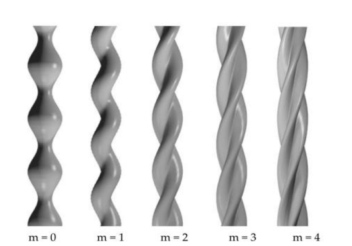
\includegraphics[width=1\linewidth]{D:/不重要过期文件/论文收集/水螺旋/不同m对应的模式}
	\caption{不同模式螺旋形状\cite{c3}}
	\label{fig:P2}%\label置于\caption后,否则可能报错
\end{figure}

由上述分析,我们得到了核心结论:\textcolor{red}{控制气体与液体流速以及气液体密度比,探究不同模式下放大率的大小来判断将产生哪种模式的扰动,由此判断是否出现水螺旋.}

\subsubsection{黏性修正}
考虑液体粘性的影响,加入修正项:
\begin{equation}
\nabla \cdot u_{1}^{'}=0
\end{equation}
\begin{equation}
\left( \frac{\partial}{\partial t}+U_1\frac{\partial}{\partial z} \right) u_{1}^{'}=-\frac{1}{\rho _1}\nabla p_1-\frac{1}{\rho _1}\nabla \cdot \tau 
\end{equation}
其中$\tau$为额外的应力张量(来自于粘滞力),对于粘弹性液体,我们引用共转八常数模型\cite{c4} ,具体可表示为如下微分方程:
\begin{equation}
\begin{split}
\tau+\lambda_{1}(\frac{\partial}{\partial t}+U_{1} \frac{\partial}{\partial z}) \tau=-\eta_{0}[\dot{\gamma}\\
+\lambda_{2}(\frac{\partial}{\partial t}+U_{1} \frac{\partial}{\partial z}) \dot{\gamma}]
\end{split}
\end{equation}
其中  $\dot{\gamma}$ 是应变张量,$\eta _0$  是零剪切粘度,$\lambda _1,\lambda _2$分别是应力松弛时间和变形延迟时间

由于我们实验用到的液体是水,水是一种牛顿流体,由此我们可以做一定的简化.

若粘弹性液体为牛顿流体,即$\lambda _1=\lambda _2=0$,且$ \eta _0=\mu =\rho v $ ,其中 $\mu$  为动态粘度, $v$   为运动粘度,于是色散方程可以化为:
\begin{equation}
\begin{gathered}
\begin{split}
(\alpha+\mathrm{i} k {U}_{1})^{2}+2 v k^{2}[\frac{I_{m}^{\prime \prime}(k a)}{I_{m}(k a)}\frac{C_{3}}{C_{1}} \frac{2}{k a}
[l a \frac{I_{m}^{\prime \prime}(l a)}{I_{m}(l a)}\\
-\frac{I_{m}^{\prime}(l a)}{I_{m}(l a)}] \frac{I_{m}^{\prime}(k a)}{I_{m}(k a)}
-\frac{C_{4}}{C_{1}} \frac{2 k l}{l^{2}+k^{2}} \frac{I_{m}^{\prime \prime}(l a)}{I_{m}^{\prime}(l a)} \frac{I_{m}^{\prime}(k a)}{I_{m}(k a)}]
\\(\alpha+\mathrm{i} k {U}_{1}) 
-\frac{C_{2}}{C_{1}} \frac{\rho_{\mathrm{g}}}{\rho} \frac{l^{2}-k^{2}}{l^{2}+k^{2}} \frac{K_{m}(k a)}{K_{m}^{\prime}(k a)}\\
 \frac{I_{m}^{\prime}(k a)}{I_{m}(k a)}\left(\alpha+\mathrm{i} k {U}_{1}{\mathrm{g}}\right)^{2}=\\
\frac{C_{2}}{C_{1}} \frac{\sigma k}{\rho a^{2}} \frac{l^{2}-k^{2}}{l^{2}+k^{2}}t(1-k^{2} a^{2}-m^{2}) \frac{I_{m}^{\prime}(k a)}{I_{m}(k a)} 
\end{split}
\end{gathered}
\end{equation}
其中的参数:
\begin{figure}[!htbp]%
	\centering
	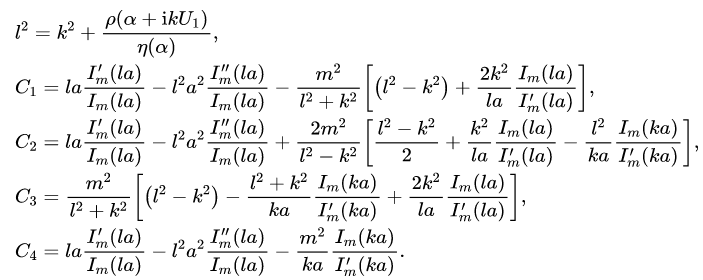
\includegraphics[width=1.2\columnwidth]{images/参数}
	\caption{参数表}
	\label{fig:P2}%\label置于\caption后,否则可能报错
\end{figure}
\subsubsection{总结}
\begin{figure}[h]%
	\centering
	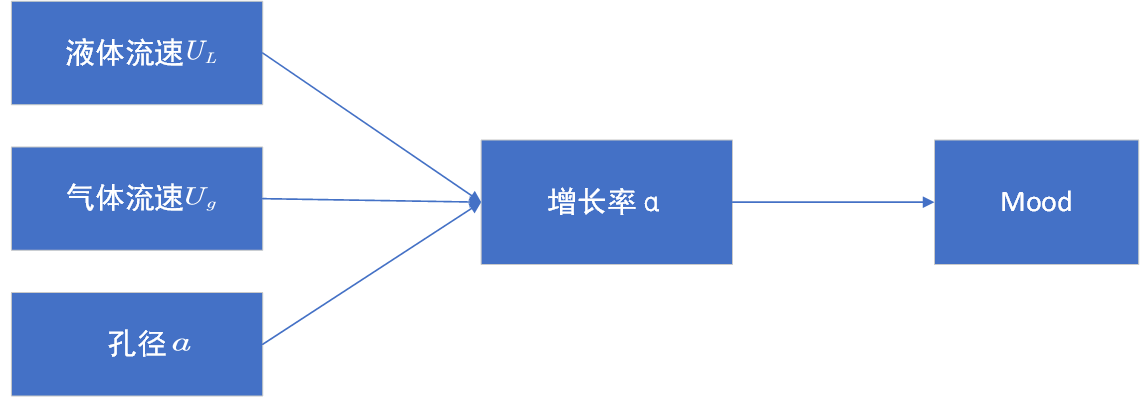
\includegraphics[width=1.2\columnwidth]{images/流程图1}
	\caption{总结流程图}
	\label{fig:P2}%\label置于\caption后,否则可能报错
\end{figure}

由此,我们总结出水螺旋产生的物理本质是:\textcolor{red}{液体的惯性力与空气对其表面张力的相互竞争.}
\section{实验}
\label{sec:Experiment}
\subsection{实验思路}
\begin{figure}[h]%
	\centering
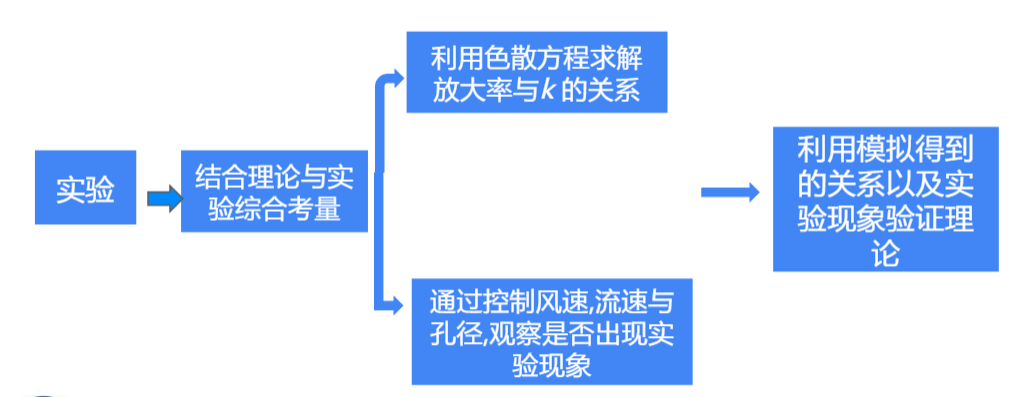
\includegraphics[width=1.2\columnwidth]{images/实验流程图}
	\caption{实验流程图}
	\label{fig:P2}%\label置于\caption后,否则可能报错
\end{figure}
\begin{figure}[h]%
	\centering
	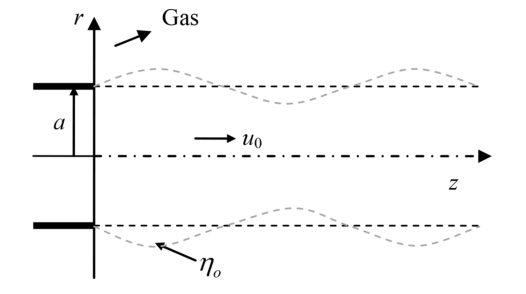
\includegraphics[width=1.2\columnwidth]{D:/不重要过期文件/论文收集/水螺旋/实验图}
	\caption{实验设计图\cite{c3}}
	\label{fig:P2}%\label置于\caption后,否则可能报错
\end{figure}

实验思路:将液体从半径为$a$的小孔中射出,控制其速度为$u_{0}$,并控制其射出的方向竖直向下.同时注入速度为$u_{1}$同轴气体,通过控制液体流速,改变气体流速,观察是否会出现螺旋的现象.
\subsection{实验器材}

通过鼓风机进行鼓风,同时利用水泵进行抽水,使水从水管流出,同时鼓风机给予同轴风速,利用风速计测量平均风速,利用量筒结合拍视频拆帧的方法测量水的流速.

\begin{figure}[!htbp]%
	\centering
	\includegraphics[width=0.6\columnwidth]{D:/不重要过期文件/论文收集/水螺旋/风速计}
	\caption{鼓风机}
	\label{fig:P2}%\label置于\caption后,否则可能报错
\end{figure}
\begin{figure}[!htbp]%
	\centering
	\includegraphics[width=0.5\columnwidth]{D:/不重要过期文件/论文收集/水螺旋/量筒}
	\caption{量筒}
	\label{fig:P2}%\label置于\caption后,否则可能报错
\end{figure}
\begin{figure}[!htbp]%
	\centering
	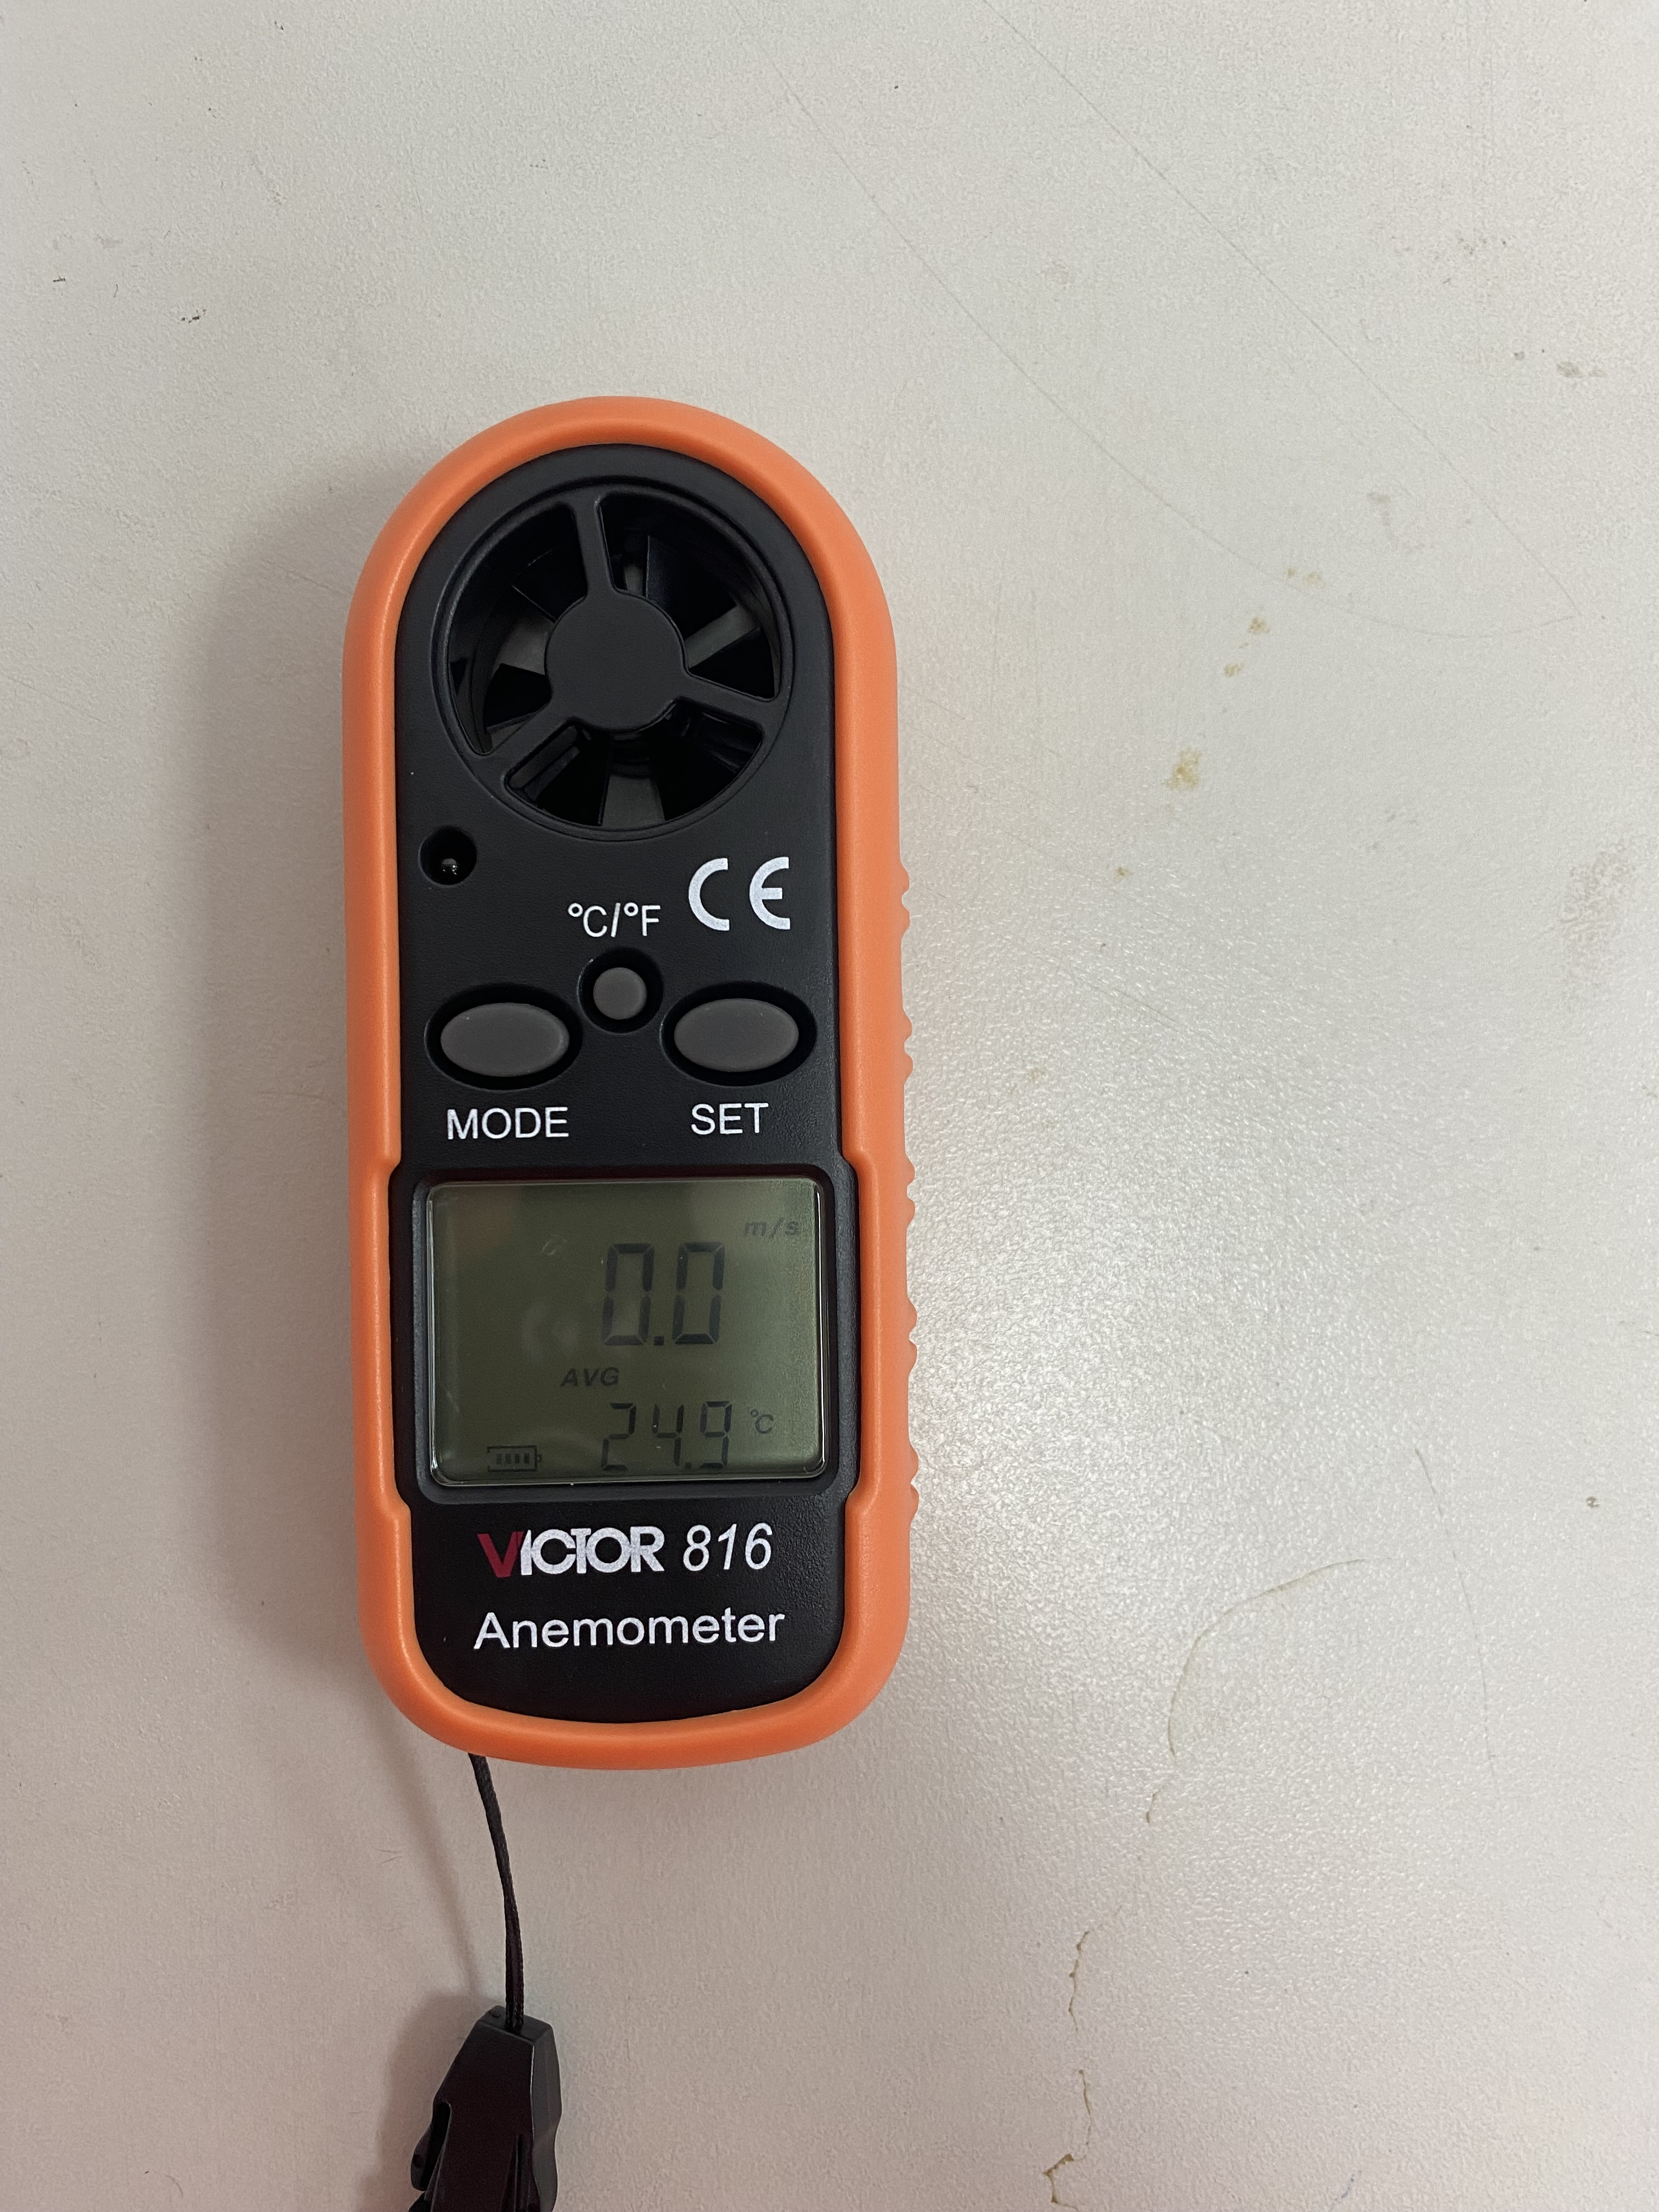
\includegraphics[width=0.6\columnwidth]{D:/不重要过期文件/论文收集/水螺旋/风速计1}
	\caption{风速计,相对误差$		\pm 5\%		$}
	\label{fig:P2}%\label置于\caption后,否则可能报错
\end{figure}
\begin{figure}[!htbp]%
	\centering
	\includegraphics[width=0.6\columnwidth]{D:/不重要过期文件/论文收集/水螺旋/水泵}
	\caption{水泵}
	\label{fig:P2}%\label置于\caption后,否则可能报错
\end{figure}
\begin{figure}[!htbp]%
	\centering
	\includegraphics[width=0.6\columnwidth]{D:/不重要过期文件/论文收集/水螺旋/水管}
	\caption{特制水管}
	\label{fig:P2}%\label置于\caption后,否则可能报错
\end{figure}
\begin{figure}[!htbp]%
	\centering
	\includegraphics[width=0.8\columnwidth]{D:/不重要过期文件/论文收集/水螺旋/实验装置}
	\caption{实验装置}
	\label{fig:P2}%\label置于\caption后,否则可能报错
\end{figure}

\subsection{实验结果}
1.孔径$2a=(5.216\pm0.242)mm$,液体流速$U_{L}=1.28m/s$,气体流速$U_{g}=2.2m/s$
\begin{figure}[H]
	\centering
	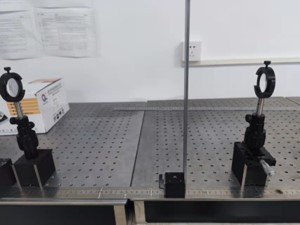
\includegraphics[width=1\linewidth]{D:/不重要过期文件/论文收集/水螺旋/22}
	\caption{数值模拟图}
	\label{fig:P2}
\end{figure}
\begin{figure}[H]
	\centering
	\includegraphics[width=0.5\linewidth,height=0.2\textheight]{D:/不重要过期文件/论文收集/水螺旋/流速1.28}
	\caption{实验图}
	\label{fig:P2}
\end{figure}

此时可以看出,在相对流速较小时,几乎没有螺旋现象产生.

2.孔径$2a=(10.628 \pm0.395)mm$ ,液体流速$U_{L}=0.603m/s$      ,气体流速$U_{g}=4.5m/s$
\begin{figure}[H]
	\centering
	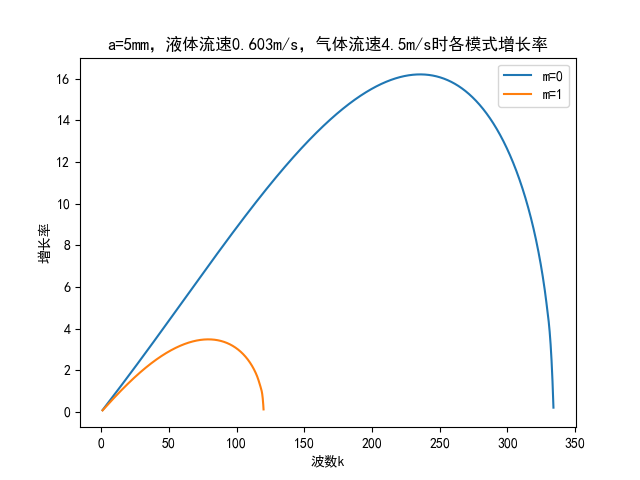
\includegraphics[width=1\linewidth]{D:/不重要过期文件/论文收集/水螺旋/45}
	\caption{数值模拟图}
	\label{fig:P2}
\end{figure}
\begin{figure}[H]
	\centering
	\includegraphics[width=0.5\linewidth,height=0.2\textheight]{D:/不重要过期文件/论文收集/水螺旋/孔径10mm,气体4.5,流速0.603}
	\caption{实验图}
	\label{fig:P2}
\end{figure}

当我们逐步增加相对流速时,能发现出现了较为明显的螺旋现象,从数值模拟和图像上我们能大致判断其为一阶螺旋.

\subsection{实验改进}

在使用上述装置进行实验时,由于使用了多管相连的结构,造成了其中的风速在传递的过程中有较大的损失,风速较低导致了相对流速较低,无法观察到一阶以上螺旋的现象.并且在出风口处,存在明显风速分布不均匀的现象.于是我们对实验装置进行了改进.

利用inventor建模,采用3D打印的方式制作了如下装置来代替之前的多管相连的结构.
\begin{figure}[H]
	\centering
	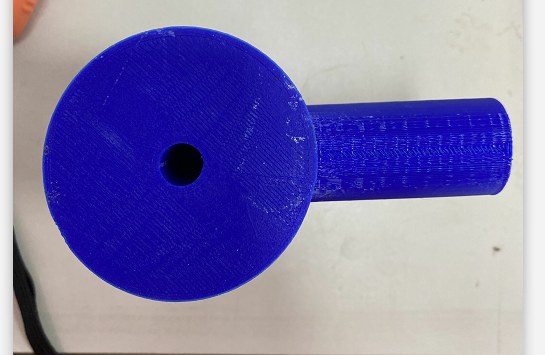
\includegraphics[width=0.8\linewidth]{images/蓝头1}
	\caption{装置进水口}
	\label{fig:P2}
\end{figure}
\begin{figure}[H]
	\centering
	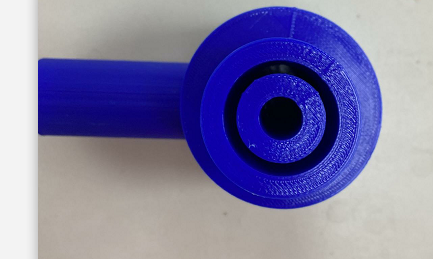
\includegraphics[width=0.8\linewidth]{images/蓝头2}
	\caption{装置出水口}
	\label{fig:P2}
\end{figure}
\begin{figure}[H]
	\centering
	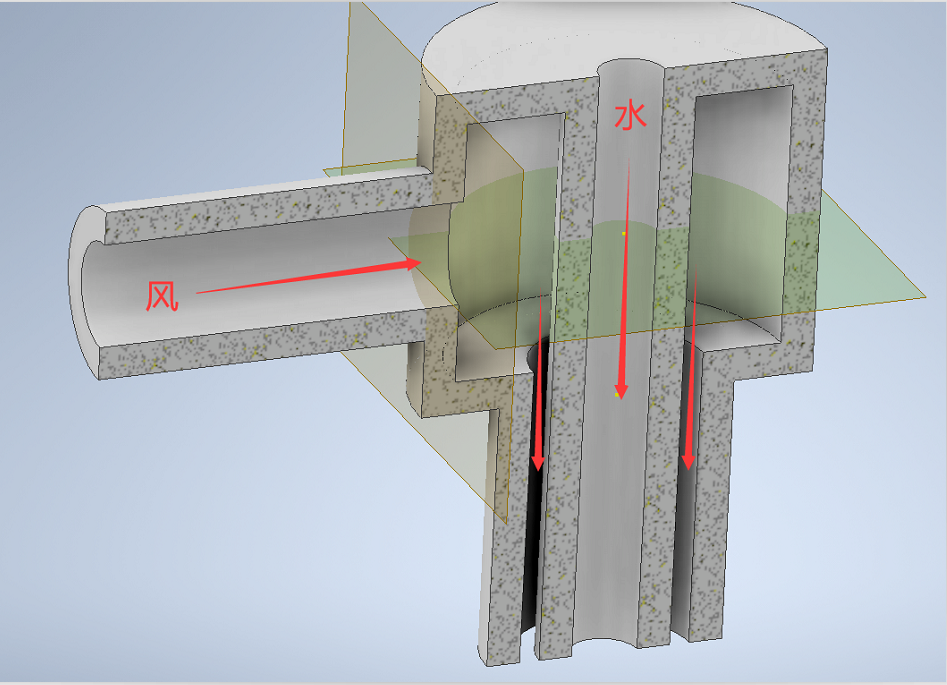
\includegraphics[width=0.8\linewidth]{images/剖面图}
	\caption{剖面图}
	\label{fig:P2}
\end{figure}

使用该装置,风速损失较小,且可以使得流下的液体受到风的扰动更加均匀.使用该装置我们搭建新的实验装置.
\begin{figure}[H]
	\centering
	\includegraphics[width=0.8\linewidth]{D:/不重要过期文件/论文收集/水螺旋/实验装置3}
	\caption{新实验装置}
	\label{fig:P2}
\end{figure}
\begin{figure}[H]
	\centering
	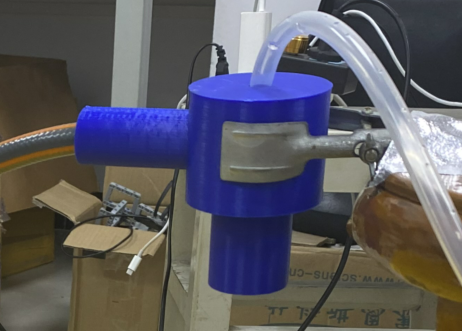
\includegraphics[width=0.8\linewidth]{D:/不重要过期文件/论文收集/水螺旋/特写}
	\caption{新实验装置特写}
	\label{fig:P2}
\end{figure}

\textbf{预实验}

在实验过程中,鼓风机会发生剧烈振动,需要通过实验检验其是否会对实验产生影响,做法如下.

将鼓风机通风口绑在装置上方,这样控制了原有的实验环境,同时未通入气体。通过观察此情况下流出液体的形状判断鼓风机的振动是否对实验产生影响. 

\begin{figure}[H]
	\centering
	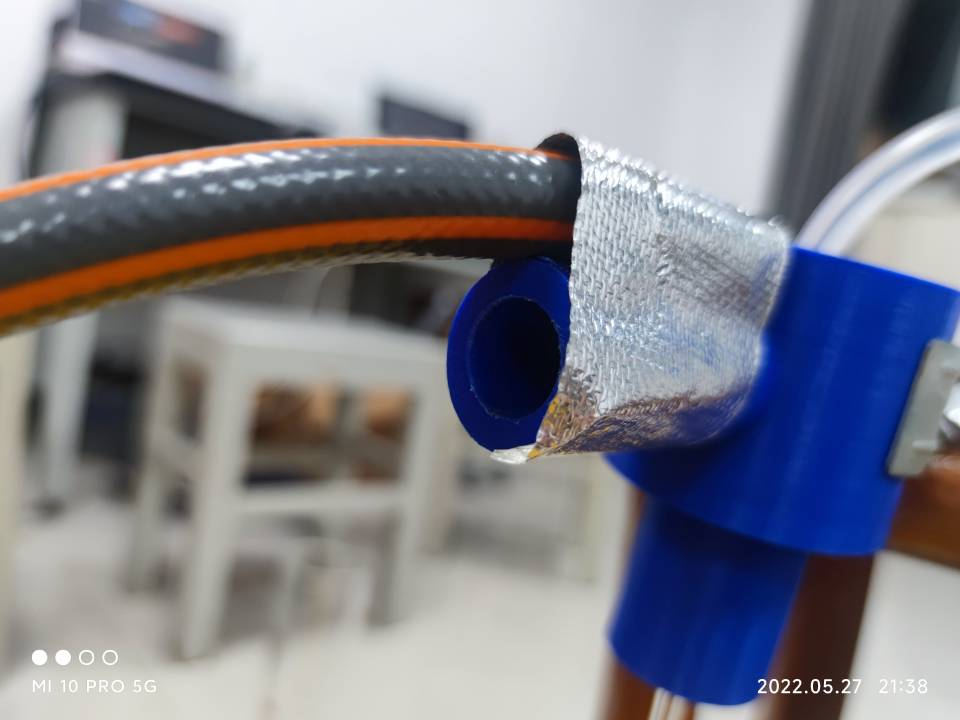
\includegraphics[width=0.8\linewidth]{D:/不重要过期文件/论文收集/水螺旋/预实验1}
	\caption{预实验装置}
	\label{fig:P2}
\end{figure}
\begin{figure}[H]
	\centering
	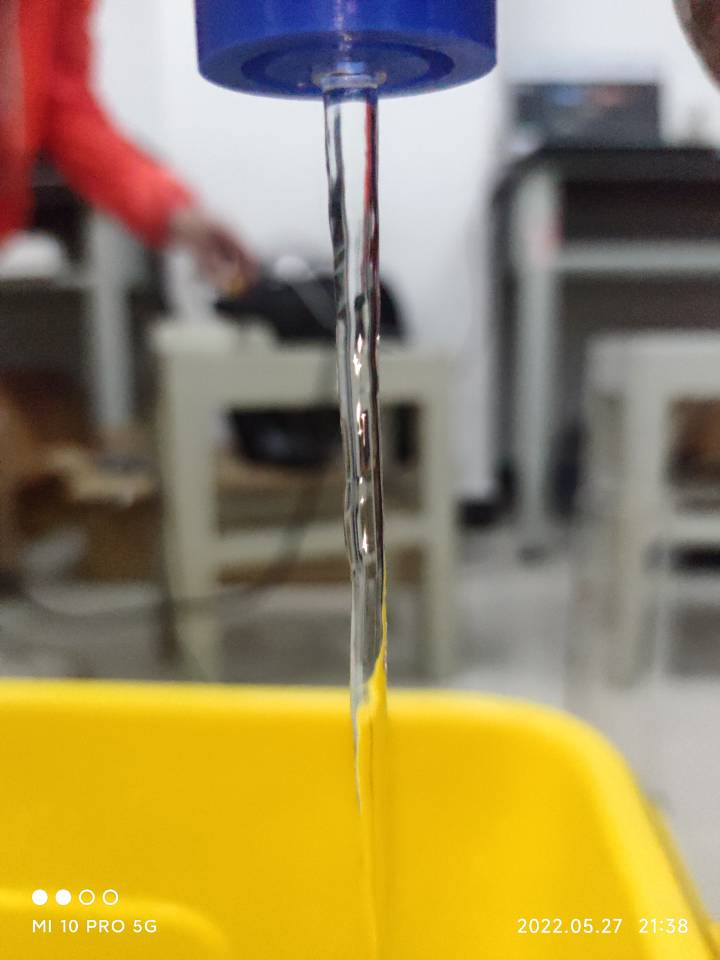
\includegraphics[width=0.5\linewidth,height=0.2\textheight]{D:/不重要过期文件/论文收集/水螺旋/预实验结果}
	\caption{预实验结果}
	\label{fig:P2}
\end{figure}

利用预实验,基本能够排除环境因素对于实验的影响.

\subsection{改进后的实验结果分析}

\textbf{1.孔径$2a=(8.064 \pm 0.191)mm$,液体流速$U_{L}=1.04m/s$ ,气体流速$U_{g}=2.4m/s$,波数$k \approx60.6m^{-1}$}
\begin{figure}[H]
	\centering
	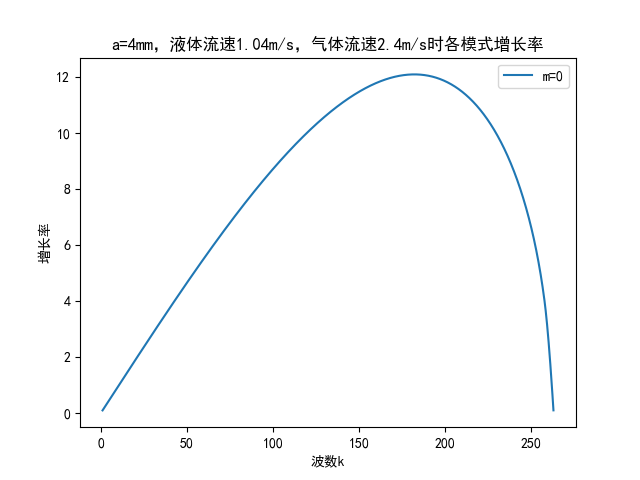
\includegraphics[width=1\linewidth]{D:/不重要过期文件/论文收集/水螺旋/Figure_3(2)}
	\caption{数值模拟图}
	\label{fig:P2}
\end{figure}
\begin{figure}[H]
	\centering
	\includegraphics[width=0.5\linewidth,height=0.2\textheight]{D:/不重要过期文件/论文收集/水螺旋/气体2.4 2}
	\caption{实验图}
	\label{fig:P2}
\end{figure}

在相对流速较低时,与之前相同,几乎没有螺旋现象产生.

\textbf{2.孔径$2a=(8.064 \pm 0.191)mm$,液体流速$U_{L}=0.554m/s$            ,气体流速$U_{g}=5.9m/s$                   ,波数 $k \approx46.9m^{-1}$}
\begin{figure}[H]
	\centering
	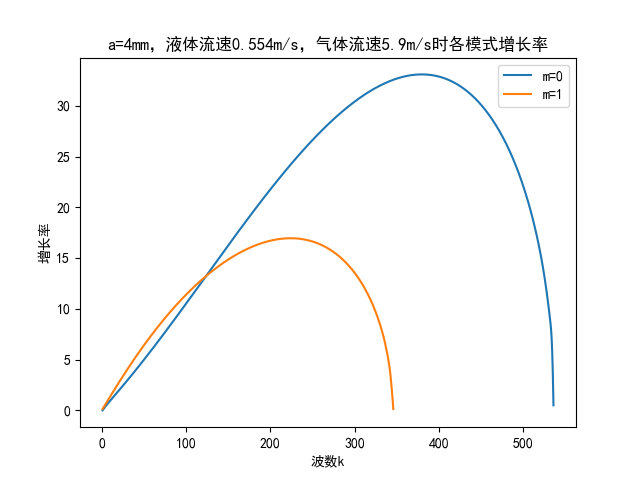
\includegraphics[width=1\linewidth]{D:/不重要过期文件/论文收集/水螺旋/59}
	\caption{数值模拟图}
	\label{fig:P2}
\end{figure}
\begin{figure}[H]
	\centering
	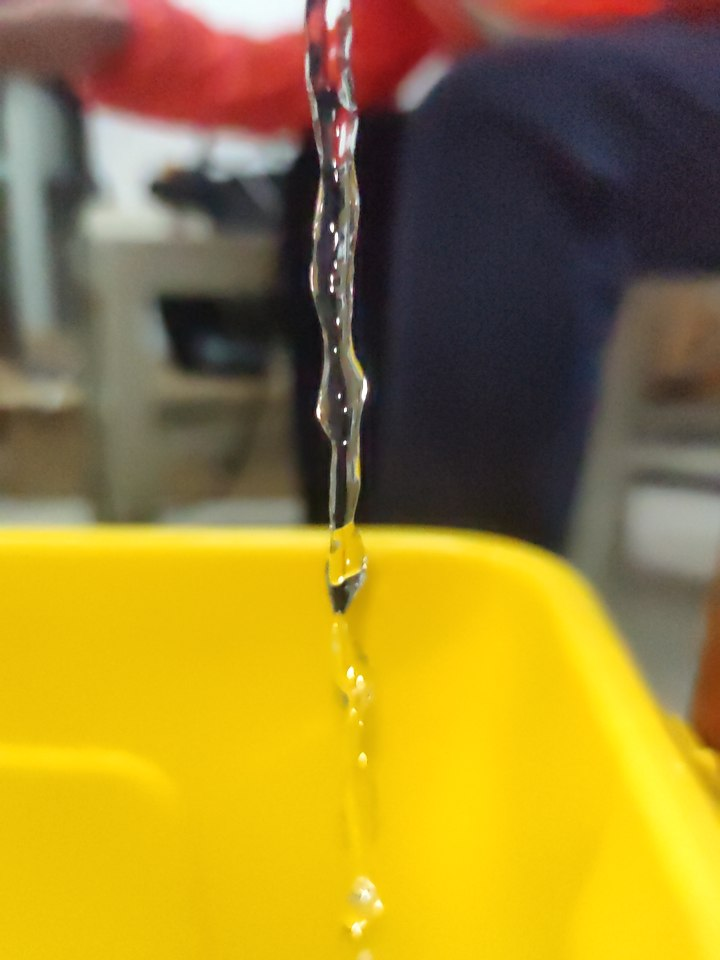
\includegraphics[width=0.5\linewidth,height=0.2\textheight]{D:/不重要过期文件/论文收集/水螺旋/5.9 2}
	\caption{实验图}
	\label{fig:P2}
\end{figure}   

当我们增加了相对流速之后,出现了螺旋现象,从模拟与图形来看,大致是产生了一阶螺旋,但由于增长率较小的原因,所以螺旋现象不是特别明显.

\textbf{3.孔径$2a=(8.064 \pm 0.019)mm$,液体流速 $U_{L}=0.777m/s$                     ,气体流速$U_{g}=11m/s$                  }
\begin{figure}[H]
	\centering
	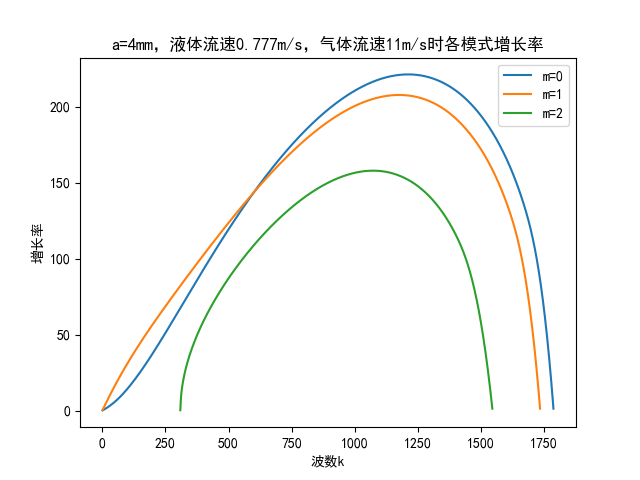
\includegraphics[width=1\linewidth]{D:/不重要过期文件/论文收集/水螺旋/Figure_4}
	\caption{数值模拟图}
	\label{fig:P2}
\end{figure}
\begin{figure}[H]
	\centering
	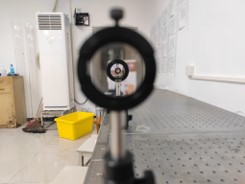
\includegraphics[width=0.5\linewidth,height=0.2\textheight]{D:/不重要过期文件/论文收集/水螺旋/11}
	\caption{实验图}
	\label{fig:P2}
\end{figure}    

当相对流速较大后,出现了非常明显的螺旋现象,从模拟和图形判断,该螺旋属于多阶螺旋混合产生的螺旋,由于拍摄技术的限制,我们难以判断其波数的大小.

\subsection{总结}
对上述的三种情况进行总结:
\begin{table}[H]
\begin{tabular}{|c|r|l}\hline
相对风速&实验结果	\\ \hline
相对低风速&几乎没有螺旋出现\\\hline
相对中风速&有一阶螺旋出现\\\hline
相对高风速&存在多阶螺旋混合出现\\\hline
\end{tabular}
\caption{实验总结}
\end{table}

\textcolor{red}{结论:相对流速越大越容易产生螺旋}
\subsection{误差分析}

可能的误差来源:
\begin{enumerate}
	\item 风速计与量筒的测量存在误差.风速的误差为$	\pm 5\%	$,量筒拆帧计算的流速的误差可用极限不确定度表示.
	\item 风速给的不一定均匀,不同方向的风速可能存在一定差别,风速计测量的仅仅是平均风速.
	\item 从照片中观察的波数不一定准确,存在误差,且在高风速情形下难以测量.
\end{enumerate}

\subsection{展望}
\begin{enumerate}
	\item 目前仅仅考虑了牛顿流体(水),还未考虑非牛顿流体的情况.
	\item 以目前的拍摄技术不太能分辨不同形式的螺旋.
	\item 暂时对其它变量考虑的比较少,仅考虑了孔径,液体流速以及气体流速的影响.
	\item 波数在风速较快时凭借现有的摄影技术难以测量.
\end{enumerate}      
%致谢,参考文献与背景信息部分=========================================================
\section*{致谢}
探究小组成员:谭帆驰\quad  丁俊翔\quad  杨超毅\quad  杜溪翔 \quad 邱卓伦  

此外,尤其鸣谢物理实验创新基地(IBPE)的各成员的协作,比赛主办方和指导老师,以及参赛同学。
%致谢部分记得改过来好吗!!!!仔细看看模板的内容!!!!!!!!!!!!!!!!!!


%背景信息
\Note{BlueNoteBackground}{
  {\textbf{Your Name}} 谭帆驰\\
  {\textbf{Address:}} 华中科技大学物理学院物理2002班\\
  {\textbf{Email:}} U202010215@hust.edu.cn
}
%写上你们的背景信息呀!!!!!!这上面的背景信息都是乱填的呀!!!!!!!!!!!
%觉得多余的可以删去,觉得不够的也可以增添别的背景信息!!!!!!!!!!!!!!!!!!!!!!!!!!!!

\section*{参考文献}
\begin{thebibliography}{2}

\bibitem{c1}Yang H Q.
\textit{Asymmetric instability of a liquid }jet[J].Physics of Fluids A,1992,4(4):681-689 

\bibitem{c2}严春吉,解茂昭. \textit{液体射流扰动控制方程边界条件及稳定性分析}, [A] 工程 数学学报 

\bibitem{c3} Xin-Tao Wang , Zhi Ning , Ming Lü.\textit{Temporal analysis of a non-Newtonian liquid jet in a compressible gas}[J]Journal of Non-Newtonian Fluid Mechanics 

\bibitem{c4}Zhihao Liu , Zhengbai Liu.\textit{Instability of a viscoelastic liquid jet with axisymmetric and asymmetric disturbances}[J]International Journal of Multiphase Flow

\bibitem{c5}曾显奎,孙志刚.\textit{液体射流在同向气流中的破裂}[A]化学工程
\end{thebibliography}

%\end{CJK}
\end{document}
